\documentclass[10pt,a4paper]{article}
\usepackage[latin1]{inputenc}
\usepackage{amsmath}
\usepackage{amsfonts}
\usepackage{amssymb}
\usepackage{hyperref}
\usepackage{graphicx}
\usepackage{cite}
%\usepackage[style=nature, backend=biber]{biblatex}
%\addbibresource{./bibfile.bib}
\DeclareMathOperator*{\argmax}{argmax} % no space, limits underneath in displays

\begin{document}
	\title{Natural Language Processing for tasks with specialized domain language  --  Project Report}
	\author{data.camp097@audi.de}
	\maketitle
	
	\section{Definition}
	\subsection{Overview}
	or Introduction or Context
	\subsection{Problem Statement}
	
	\subsection{Metrics}
	\section{Analysis}
	\subsection{The Dataset}
	The dataset chosen for this project consists of three different sources:
		\begin{itemize}
		\item technical / specialist books: 60 titles, 28507 pages, 5950125 words in total 
		\item internal technical documentation: 17763 change requests for embedded control software with a total of 960921 words\footnote{proprietary, cannot be submitted} 
		\item patents: 500 patents from the domain vehicle powertrain, containing a total of 9871 pages with a total of 3929993 words.
	\end{itemize}
    \subsection{Algorithms}
    \subsection{Benchmark Models}
    As a benchmark I chose the pretrained German Facebook FastText embedding. \footnote{\url{www.spiegel.de}}
	\subsection{Related Work}
	Overview over the word embeddings used:
	\begin{center}
		\begin{tabular}{|l|p{3cm}| p{3cm}| p{3cm}|}
			\hline
			\textbf{Word Embedding} & pretrained & trained & retrained \\ 
			\hline
			word2vec  & GenSim Standard & w/ GenSim Implementation & done w/ GenSim implementation \\  
			\hline
			GloVe & GenSim Standard &w/ GenSim implementation & n.a., needs global cooccurence matrix \\  
			\hline
			FastText & from Facebook-Page,  & w/ Facebook implementation & done w/ undocumented feature in Facebook implementation\\
			\hline
			 	
			
			
		\end{tabular}
	\end{center}
	\section{Methodology}
	\subsection{Data Preprocessing}
	For 
	\subsection{Implementation}
	Training the embeddings
	
	\subsection{Optimization}
	One problem seems to be overfitting to the small number of currently available labelled samples. The learning curves suggest this.
	
	To prevent overfitting, the following steps were taken:
	\begin{itemize}
		\item Early termination.
		\item Dropout. 
		\item Model Capacity. 
	\end{itemize}
    Other options that were not thoroughly explored in this project include
	\begin{itemize}
		\item Regularization.
		\item Data augmentation
		\item Acquisistion of more data.
	\end{itemize}
	\section{Results}
	\subsection{Visualizations}
	    \begin{center}
		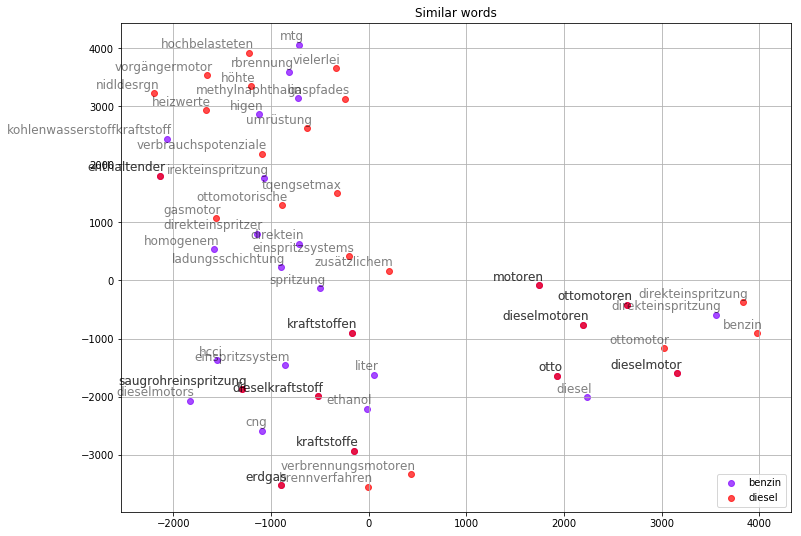
\includegraphics[scale=0.5]{./Pictures/test.png}
		\caption{Conic Section}
	\end{center}
	
	My proposed evaluation is best summarized in an empty results table:
	
	\begin{center}
		\begin{tabular}{|l| c| c| c|c|}
			\hline
			\textbf{Word Embedding} & $\boldsymbol{M_1}$ & $\boldsymbol{M_2}$ & $\boldsymbol{M_3}$ & $\boldsymbol{M_4}$\\ 
			\hline
			word2vec pretrained & \textbullet & \textbullet & \textbullet & \textbullet\\  \hline
			word2vec retrained & \textbullet & \textbullet & \textbullet & \textbullet\\  	\hline
			word2vec trained from scratch  & \textbullet & \textbullet & \textbullet & \textbullet\\  	\hline
			GloVe pretrained & \textbullet & \textbullet & \textbullet & \textbullet\\  
			\hline
			GloVe retrained & \textbullet & \textbullet & \textbullet & \textbullet\\
			\hline
			GloVe trained from scratch  & \textbullet & \textbullet & \textbullet & \textbullet\\  	
			\hline
			FastText pretrained & \textbullet & \textbullet & \textbullet & \textbullet\\  \hline
			FastText retrained & \textbullet & \textbullet & \textbullet & \textbullet\\  	\hline
			FastText trained from scratch  & \textbullet & \textbullet & \textbullet & \textbullet\\  	
			\hline
			
			
		\end{tabular}
	\end{center}
	\section{Conclusion}
	\subsection{Reflection}
	\subsection{Improvement/Future Work}
	
	
	Natural Language Processing as a sub-discipline of machine learning has had major success in recent years on a broad range of natural language related tasks. An overview of recent trends is this field can for example be found in the paper \cite{1708.02709} "Recent Trends in Deep Learning Based Natural Language Processing" by Young et al.. 
	However, when confronted with highly specialized sub-domain languages, commercial off the shelf (COTS) products decline in performance, often up to a point of being useless \cite{OilandGas}. As an example from personal experience, I would like to mention the use of Google Translate, a benchmark NLP product, on translating text from climbing guidebooks. The results are funny, but utterly useless.
	
	Another example more relevant for this work is the author's area of expertise, automotive engineering. There exist many potentially useful NLP tasks in the automotive industry, ranging from automated scanners for the monitoring of (social) media with respect to potential quality or safety problems (a legal requirement for manufacturers), automated analysis of warranty and repair documents, systems for customer support, monitoring and analysis of patent applications to identify trends and many more.
	As in the example of climbing guidebooks, the results of COTS products when confronted with this form of specialized sub-domain language are usually poor. 
	The topic of the capstone project is to make the first steps to remedy this situation. In particular, we will try to improve the word embeddings for our subdomain of interest.
	
	\section{Problem Statement}
	The basic hypothesis for this capstone project is the assumption that the dominant problem of NLP algorithms operating in highly specialized domain languages is the fact that during training the algorithm hasn't seen any or enough domain specific text. 
	One important element of most modern NLP pipelines is a dense vector representation, also referred to as word embedding, instead of sparse representations like one-hot-encoding or bag-of-words. Examples of these methods are word2vec \cite{word2vec}, GloVe \cite{pennington2014glove} or FastText \cite{bojanowski2017enriching}. I assume that in particular these representations are not trained well enough on domain-specific language. 
	
	\section{Datasets and Inputs}
	The dataset consists of 3 different types of technical documents in German:
	\begin{itemize}
		\item technical / specialist books: 60 titles, 28507 pages, 5950125 words in total 
		\item internal technical documentation: 17763 change requests for embedded control software with a total of 960921 words\footnote{proprietary, cannot be submitted} 
		\item patents: 500 patents from the domain vehicle powertrain, containing a total of 9871 pages with a total of 3929993 words.
	\end{itemize}

	This data will have to be preprocessed. Preprocessing includes cleaning the documents from things like stopwords, interpunctuation and capitalization. After this a tokenizer and lemmatizer will be used. The preprocessed text will then be used for training of the word embedding.
	
	\section{Solution Statement}
	In a word: Train word embeddings on text from the subdomain of interest.
	First I propose to review the different existing word embeddings like Word2vec, GloVe or  FastText and pick one to work with. An important part of the research will be the question of how to make sure the embedding performs well on both text in general \textbf{and} the domain language. To achive this, I aim at using some sort of pretraining. How this is done best to balance the performance is probably one of the key research questions.
	The implementation and training itself should be pretty straightforward as there are packages for many word embeddings available that I would use for this project.
	
	\section{Benchmark Model}
	As a benchmark, I propose taking an existing trained word embedding. For all the mentioned word embeddings (Word2vec, GloVe, FastText) there exist extensively pretrained models for many languages in NLP Toolkits like spacy \cite{spacy2}, gensim \cite{rehurek_lrec} or NLTK \cite{Loper:2002:NNL:1118108.1118117} or GitHub (cf. Section \ref{web_resources}). For details on how to get from a word embedding to an evaluation metric, please refer to section \ref{eval} Evaluation Metrics.
	
	\section{Evaluation Metrics}
	\label{eval}
	To the best of my knowledge, there does not exist a single commonly used or agreed upon method on how to evaluate models\cite{1901.09785, Schnabel15, 1801.09536}. Instead a range of methods is used, these methods fall in two categories, extrinsic and intrinsic. Intrinsic evaluation takes into consideration only the embedding itself whereas extrinsic methods measure the embedding performance indirectly by a downstream NLP task with its own metric.
	In this project I will use the following metrics:
	\begin{itemize}
		\item \textbf{$M_1$}: Extrinsic measure: A multiclass classification task of change requests for embedded control software will be used a an extrinsic metric. In particular, the Top 1 and Top 2 accuracy will be used to compare the word embeddings performance.\footnote{The classification task itself relies on proprietary text that cannot be published or submitted.}
		
		\item \textbf{$M_2$}: Clustering by subsystem. A vehicle is built from subsystems like engine, transmission, chassis, interior, etc. For a few different subsystems, we will each pick a list of words that belong to the subsystem. On this set of words, we can then perform clustering or classification. For word embeddings, we use the consine distance
		\begin{equation}
               d(\bold{a}, \bold{b})=\cos(\theta)=\frac{\bold{a} \cdot \bold{b}}{|\bold{a}|\cdot|\bold{b}|}
		\end{equation}
		
		With this distance measure, we can do a KNN classification and will take the resulting classification accuracy as an intrinsic measure for the word embedding.  
		
		\item \textbf{$M_3$}: Word analogy. Another intrinsic metric for word embddings is to assess semantic meaning. We look for relations of the form
	    $$ a:b::c:d $$
	    In particular, we will assess the semantic representation of technical concepts. Two examples are 
		$$\text{engine : engine control unit :: transmission : transmission control unit}$$
		$$\text{camshaft : camshaft bearing :: crankshaft : crankshaft bearing}$$
		
		We can extract the word d from words a,b and c from the embedding simply with
		\begin{equation}
		d=\argmax_{i} \frac{(x_b -x_a + x_c)^T\cdot x_i}{|x_b-x_a+x_c|}
		\end{equation}
		

	\item \textbf{$M_4$}: Word similarity. I will compile a list of pairs of words from technical jargon and ask colleagues to rate their similarity. This measure of similarity will then be compared to the cosine distance the embeddings produce for these word pairs. This metric can also be adopted to include relatedness instead of similarity.
	
	\item As a qualitative measure I intend to visualize the embedding using t-SNE \cite{vanDerMaaten2008} to get a comparative qualitative measure.
\end{itemize}
	
My proposed evaluation is best summarized in an empty results table:
	
		\begin{center}
			\begin{tabular}{|l| c| c| c|c|}
				\hline
				\textbf{Word Embedding} & $\boldsymbol{M_1}$ & $\boldsymbol{M_2}$ & $\boldsymbol{M_3}$ & $\boldsymbol{M_4}$\\ 
				\hline
				word2vec pretrained & \textbullet & \textbullet & \textbullet & \textbullet\\  \hline
			    word2vec retrained & \textbullet & \textbullet & \textbullet & \textbullet\\  	\hline
			    word2vec trained from scratch  & \textbullet & \textbullet & \textbullet & \textbullet\\  	\hline
			    GloVe pretrained & \textbullet & \textbullet & \textbullet & \textbullet\\  
			    \hline
			    GloVe retrained & \textbullet & \textbullet & \textbullet & \textbullet\\
			    \hline
			    GloVe trained from scratch  & \textbullet & \textbullet & \textbullet & \textbullet\\  	
			    \hline
			    FastText pretrained & \textbullet & \textbullet & \textbullet & \textbullet\\  \hline
			    FastText retrained & \textbullet & \textbullet & \textbullet & \textbullet\\  	\hline
			    FastText trained from scratch  & \textbullet & \textbullet & \textbullet & \textbullet\\  	
			    \hline
			    
				    
			\end{tabular}
		\end{center}
		
	where $M_i$ are the metrics as described above.
	

	\section{Additional Research Questions}
	\paragraph{Extra Dimesions.} If we retrain a word embedding for a specialized subdomain, do we need to add a few dimensions to the vector space "to make room" for additional semantic concepts? Intuitition would suggest that all existing dimensions are already somehow occupied and new technical concepts would require "new space". So an additional question would be: Do extra dimesions improce the embedding quality? And if so, what semantic meaning can we assign the new dimensions? 
	\paragraph{Compund Nouns.} A distinctive feature of the German language are compound nouns. This holds especially true for technical terms like Nockenwellenlagerungskonzept (cam shaft bearing method). I expect this to be of particular importance to be reflected in the embedding. 
	
	
		
	\section{Project Design}
	The project design  seems pretty straightforward. The steps themselves and the whole process will most likely be highly iterative.
	In a first step I will collect text for a particular specialized subdomain by collecting existing documents and scraping additional text off the internet. Where possible, I will try to leverage existing Python packages like pypatent etc. for the scraping
	In a second step, I will preprocess the collected texts as described above. For this task, I will rely on existing NLP toolkits like NLTK or gensim.
	In a third step I will use three popular word embeddings: word2vec, GloVe and FastText. These word embeddings will be used pretrained, trained from scratch and retrained. The results will be compared with the described evaluation metrics.	
	

\section{Web Resources}
\label{web_resources}
\begin{itemize}
	\item \url{https://github.com/kudkudak/word-embeddings-benchmarks/blob/master/web/datasets/similarity.py}
	\item \url{https://github.com/Hironsan/awesome-embedding-models}
	\item \url{https://github.com/philipperemy/keras-attention-mechanism}
\end{itemize}



\nocite{*}

\bibliography{Project_Report}
\bibliographystyle{ieeetr}

	
	
\end{document}